%****************************************************************************%
%* DIET User's Manual deploying chapter file                                *%
%*                                                                          *%
%*  Author(s):                                                              *%
%*    - Holly DAIL (Holly.Dail@ens-lyon.fr)                                 *%
%*    - Raphael BOLZE (Raphael.Bolze@ens-lyon.fr)                           *%
%*    - Eddy CARON (Eddy Caron@ens-lyon.fr)                                 *%
%*    - Philippe COMBES (Philippe.Combes@ens-lyon.fr)                       *%
%*    - Benjamin DEPARDON (Benjamin.Depardon@ens-lyon.fr)                   *%
%*                                                                          *%
%* $LICENSE$                                                                *%
%****************************************************************************%
%* $Id: deploy.tex,v 1.27 2011/05/02 10:01:43 bdepardo Exp $
%* $Log: deploy.tex,v $
%* Revision 1.27  2011/05/02 10:01:43  bdepardo
%* Corrected a few typos.
%* Renamed "round-robin" scheduler into "least recently used" scheduler as this
%* is closer to the behavior of this scheduler.
%*
%* Revision 1.26  2010/09/19 10:35:46  bdepardo
%* Added a section on how to choose the shape of the hierarchy
%*
%* Revision 1.25  2010/03/29 21:18:17  ecaron
%* Update GoDIET commands
%*
%* Revision 1.24  2010/02/25 08:05:27  ycaniou
%* e.g -> Use macro
%* Typo + ispell
%*
%* Revision 1.23  2010/02/25 06:45:38  ycaniou
%* Add local variables
%*
%* Revision 1.22  2010/01/21 14:05:58  bdepardo
%* DIET -> \diet
%* SeD -> \sed
%* GoDIET -> \godiet
%*
%* Revision 1.21  2008/07/16 23:02:48  ecaron
%* Fixe the problem with too long list of hosts
%*
%* Revision 1.20  2008/03/04 16:12:37  bdepardo
%* Added a link to the file examples/commented.xml for GoDIET.
%*
%* Revision 1.19  2006/11/29 16:55:49  dloureir
%* minor corrections
%*
%* Revision 1.18  2006/05/12 12:12:32  sdahan
%* Add some documentation about multi-MA
%*
%* Bug fix:
%*  - segfault when the neighbours configuration line was empty
%*  - deadlock when a MA create a link on itself
%*
%* Revision 1.17  2005/07/13 07:56:15  hdail
%* Corrected error in xml example and added console instructions to GoDIET section.
%*
%* Revision 1.16  2005/07/12 21:44:28  hdail
%* - Correcting small problems throughout
%* - Modified deployment chapter to have a real section for deploying via GoDIET
%* - Adding short xml example without the comments to make a figure in GoDIET
%*   section.
%*
%* Revision 1.15  2005/06/28 15:53:02  hdail
%* Completed corrections for config file examples and text explaining launch of
%* each component.
%*
%* Revision 1.14  2005/06/28 13:57:55  hdail
%* Described GoDIET and updating section on launching by hand.
%*
%* Revision 1.13  2005/06/24 14:27:07  hdail
%* Correcting english problems & updating descriptions that are no longer true.
%*
%* Revision 1.12  2005/06/14 08:26:32  ecaron
%* Deployment section should introduce GoDIET (Fixme for Holly)
%*
%* Revision 1.11  2005/05/29 13:51:22  ycaniou
%* Moved the section concerning FAST from description to a new chapter about FAST
%* and performances prediction.
%* Moved the section about convertors in the FAST chapter.
%* Modified the small introduction in chapter 1.
%* The rest of the changes are purely in the format of .tex files.
%*
%* Revision 1.10  2004/10/25 08:59:56  sdahan
%* add the multi-MA documentation
%*
%* Revision 1.9  2004/09/28 07:03:39  rbolze
%* remove useAsyncAPI parameter
%*
%* Revision 1.8  2004/07/12 08:33:58  rbolze
%* explain how to copy cfgs file in install_dir/etc directory and correct my english
%****************************************************************************%

\chapter{Deploying a \diet platform}
\label{ch:deploying}

Deployment is the process of launching a \diet platform including agents and
servers.  For \diet, this process includes writing configuration files for each
element and launching the elements in the correct hierarchical order. There are
three primary ways to deploy \diet.

Launching \textbf{by hand} is a reasonable way to deploy \diet for small-scale
testing and verification. This chapter explains the  necessary services, how to
write \diet configuration files, and in what order \diet elements should be
launched.  See Section~\ref{sec:deployBasics} for details.

\textbf{\godiet} is a Java-based tool for automatic \diet deployment that
manages configuration file creation, staging of files, launch of elements,
monitoring and reporting on launch success, and process cleanup when the \diet
deployment is no longer needed.   See  Section~\ref{sec:deployGoDIET} for
details.

\textbf{Writing your own scripts} is a surprisingly popular approach.  This
approach often looks easy initially, but can sometimes take much, much longer
than you predict as there are many complexities to manage.  Learn \godiet -- it
will save you time!



\section{Deployment basics}
\label{sec:deployBasics}


\section{\godiet}
\label{sec:deployGoDIET}

%%Description
\godiet is an cross-platform tool that helps you automate ad-hoc deployment and
management procedures for \diet infrastructure. It manages
configuration file creation, staging of files, launch of elements, monitoring
and reporting.  \godiet is extremely useful for large deployments on a complex
physical infrastructure. The mains features are:
\begin{itemize}
  \item Complete command line interface.
  \item Distributed command execution via SSH.
  \item Real time monitoring applications state.
  \item Complex physical infrastructure management with firewall and multiple
    network lan.
\end{itemize}
\begin{figure}[h]
  \centering
  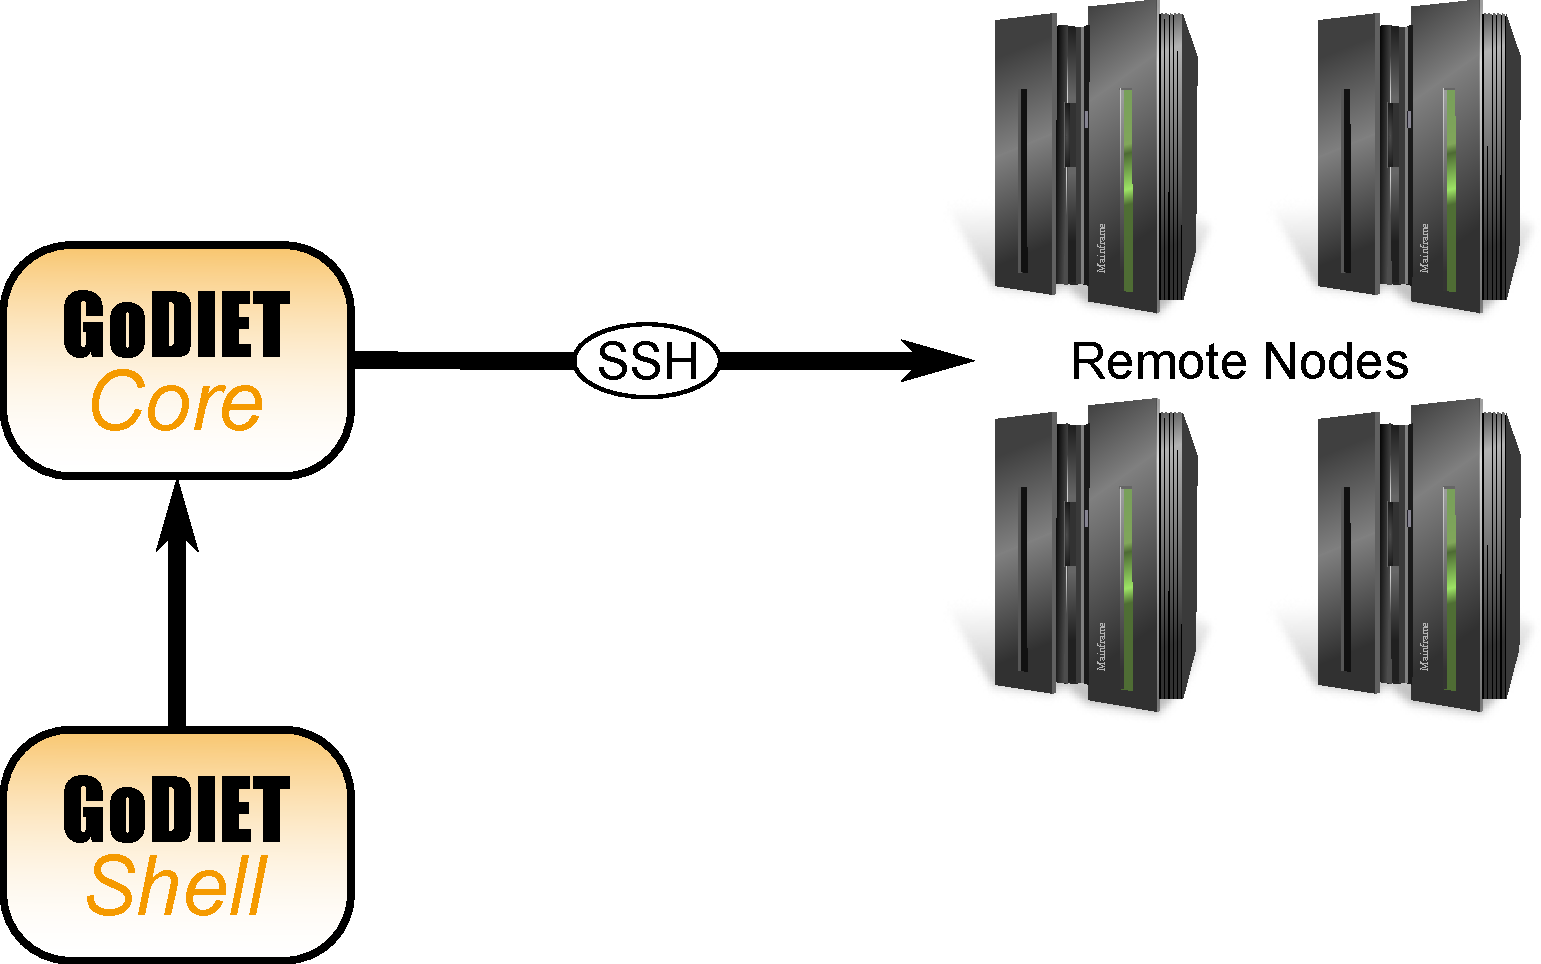
\includegraphics[width=16cm]{fig/schemaPhilippe}
  \caption{Design principle of \godiet.\label{fig:GODIETDesign}}
\end{figure}




\subsection{Installing GoDiet}

The following operating systems are known to support GoDiet:
\begin{itemize}
    \item Linux: Most recent distributions are likely to work
    \item Mac OS X 10.4 or later
\end{itemize}

You need to have the Sun Java 6 or OpenJDK6 installed. All operating system with Java 6 must support 
First download \godiet on the project website\footnote{http://graal.ens-lyon.fr/DIET/godiet.html}.

 Extract the archive just and launch run.bat or run.sh script.
You need to load your physical platform on which will \godiet will
running. This platform must be describe in a XML file based on
\textit{Platform.xsd} grammar. You can find an simple file in the example directory 

\subsection{Godiet input}

\godiet needs input data to work.  Currently the 
\subsubsection{Infrastructure}
\label{GODIETInfrastructureDesc}
%%Physical platform
The user also defines all machines available for the deployment, disk scratch
space available at each site for storage of configuration files, and which
machines share the same disk to avoid unecessary copies. 

\subsubsection{Diet platform}
\label{GODIETPlatformDesc}
%%Platform Diet
The user of \godiet could describes the desired
deployment in an XML file including all needed external services (\eg omniNames
and LogService); the desired hierarchical organization of agents and servers is
expressed directly using the hierarchical organization of XML. 

\subsection{Godiet commands}

\subsubsection{Help}

\subsubsection{SSH}

\subsubsection{Load}

\subsubsection{Start & Stop}

\subsubsection{Status}

\subsubsection{Draw}

An example input XML file is shown in Figure~\ref{fig:godietXml}; see
\cite{CDa05} for a full explanation of all entries in the XML. You can also
have a look at the fully commented XML example file provided in the \godiet
distribution under examples/commented.xml, each option is explained. To launch
\godiet for the simple example XML file provided in the \godiet distribution
under examples/example1.xml, run:

\begin{verbatim}
~ > java -jar GoDIET-x.x.x.jar example1.xml
XmlScanner constructor
Parsing xml file: example1.xml
GoDIET>
\end{verbatim}

\godiet reads the XML file and then enters an interactive console mode. In this
mode you have a number of options:

%% \begin{verbatim}
%% GoDIET> help
%% The following commands are available:
%%    launch:       launch entire DIET platform
%%    launch_check: launch entire DIET platform then check its status
%%    relaunch:     kill the current platform and launch entire DIET platform once again
%%    stop:         kill entire DIET platform using kill pid
%%    status:       print run status of each DIET component
%%    history:      print history of commands executed
%%    help:         print this message
%%    check:        check the platform status
%%    stop_check:   stop the platform status then check its status before exit
%%    exit:         exit GoDIET, do not change running platform.
%% \end{verbatim}

We will now launch this example; note that this example is intentionally very
simple with all components running locally to provide initial familiarity with
the \godiet run procedure. Deployment with \godiet is especially useful  when
launching components on multiple remote machines.

\begin{verbatim}
GoDIET> launch
* Launching DIET platform at Wed Jul 13 09:57:03 CEST 2005

Local scratch directory ready:
        /home/hdail/tmp/scratch_godiet

** Launching element OmniNames on localHost
Writing config file omniORB4.cfg
Staging file omniORB4.cfg to localDisk
Executing element OmniNames on resource localHost
Waiting for 3 seconds after service launch

** Launching element MA_0 on localHost
Writing config file MA_0.cfg
Staging file MA_0.cfg to localDisk
Executing element MA_0 on resource localHost
Waiting for 2 seconds after launch without log service feedback

** Launching element LA_0 on localHost
Writing config file LA_0.cfg
Staging file LA_0.cfg to localDisk
Executing element LA_0 on resource localHost
Waiting for 2 seconds after launch without log service feedback

** Launching element SeD_0 on localHost
Writing config file SeD_0.cfg
Staging file SeD_0.cfg to localDisk
Executing element SeD_0 on resource localHost
Waiting for 2 seconds after launch without log service feedback
* DIET launch done at Wed Jul 13 09:57:14 CEST 2005 [time= 11.0 sec]
\end{verbatim}

The \texttt{status} command will print out the run-time status of all launched
components. The \texttt{LaunchState} reports whether \godiet observed any
errors during the launch itself. When the user requests the launch of
LogService in the input XML file, \godiet can connect to the LogService  after
launching it to obtain the state of launched components; when available, this
state is reported in the \texttt{LogState} column.

\begin{verbatim}
GoDIET> status
Status   Element   LaunchState   LogState   Resource     PID
         OmniNames running       none       localHost    1232
         MA_0      running       none       localHost    1262
         LA_0      running       none       localHost    1296
         SeD_0     running       none       localHost    1329
\end{verbatim}

Finally, when you are done with your \diet deployment you should always run
\texttt{stop}. To clean-up each element, \godiet runs a \texttt{kill} operation
on the appropriate host using the stored PID of that element.

\begin{verbatim}
GoDIET> stop

* Stopping DIET platform at Wed Jul 13 10:05:42 CEST 2005
Trying to stop element SeD_0
Trying to stop element LA_0
Trying to stop element MA_0
Trying to stop element OmniNames

* DIET platform stopped at Wed Jul 13 10:05:43 CEST 2005[time= 0.0 sec]
* Exiting GoDIET. Bye.
\end{verbatim}

\begin{figure}[p]
%****************************************************************************%
%* DIET User's Manual xml file for deployment chapter                       *%
%*                                                                          *%
%*  Author(s):                                                              *%
%*    - Holly DAIL (Holly.Dail@ens-lyon.fr)                                 *%
%*    - Raphael BOLZE (Raphael.Bolze@ens-lyon.fr)                           *%
%*                                                                          *%
%* $LICENSE$                                                                *%
%****************************************************************************%
%* $Id: xml_example.tex,v 1.4 2010/03/29 23:13:54 ecaron Exp $ 
%* $Log: xml_example.tex,v $
%* Revision 1.4  2010/03/29 23:13:54  ecaron
%* Update for DIET 2.4
%*
%* Revision 1.3  2006/10/31 21:29:58  ecaron
%* XML file example for Deployment chapter in DIET User's Manual
%* 
%****************************************************************************%


\lstset{language=XML, 
        basicstyle=\tiny, 
        keywordstyle=\bfseries,
        showspaces=false,
        showtabs=false,
        emphstyle=\bfseries,
        morecomment=[s][\mdseries\slshape]{<!--}{-->},
        breaklines, 
        postbreak=\space}

\begin{lstlisting}
<?xml version="1.0" standalone="no"?>
<!DOCTYPE diet_configuration SYSTEM "../GoDIET.dtd">
<diet_configuration>
  <goDiet debug="2" saveStdOut="yes" saveStdErr="yes" useUniqueDirs="no" log="no"/>
  <resources>
    <scratch dir="/tmp/GoDIET_scratch"/>
    <storage label="disk-1">
        <scratch dir="/tmp/run_scratch"/>
        <scp server="res1" login="doe"/>
    </storage>
    <storage label="disk-2">
        <scratch dir="/tmp/run_scratch"/>
        <scp server="res2" login="foo"/>
    </storage>
    <storage label="disk-3">
        <scratch dir="/tmp/run_scratch"/>
        <scp server="res3" login="bar"/>
    </storage>
    <compute label="res1" disk="disk-1">
        <ssh server="res1" login="doe"/>
	<env>
	      <var name="PATH" value=""/>
	      <var name="LD_LIBRARY_PATH" value=""/>
	</env>
    </compute>
    <compute label="res2" disk="disk-2">
        <ssh server="res2" login="foo"/>
	       <env>
		       <var name="PATH" value=""/>
		       <var name="LD_LIBRARY_PATH" value=""/>
	       </env>
    </compute>
	<cluster label="res3" disk="disk-3" login="bar">
      <env> 
      	<var name="PATH" value=""/>
        <var name="LD_LIBRARY_PATH" value=""/>
      </env>
      <node label="res3_host1">
        <ssh server="host1.res3.fr"/> 
        <end_point contact="192.5.80.103"/>
      </node>
      <node label="res3_host2">
        <ssh server="host2.res3.fr"/>
      </node>
    </cluster>
  </resources>
  <diet_services>
	  <omni_names contact="res1_IP" port="2121">
        <config server="res1" remote_binary="omniNames"/>
    </omni_names>
  </diet_services>
  <diet_hierarchy>
    <master_agent label="MA">
        <config server="res1" remote_binary="dietAgent"/>
           <cfg_options>
	     <option name="traceLevel" value="1"/>
	   </cfg_options>
            <SeD label="SeD1">
                <config server="res2" remote_binary="server_dyn_add_rem"/>
           <cfg_options>
	     <option name="traceLevel" value="1"/>
	   </cfg_options>
            </SeD>
        <SeD label="SeD2">
            <config server="res3_host1" remote_binary="server_dyn_add_rem"/>
           <cfg_options>
	     <option name="traceLevel" value="30"/>
	   </cfg_options>
	   <parameters string="T"/>
        </SeD>
        <SeD label="SeD3">
            <config server="res3_host2" remote_binary="server_dyn_add_rem"/>
           <cfg_options>
	     <option name="traceLevel" value="1"/>
	   </cfg_options>
        </SeD>
    </master_agent>
  </diet_hierarchy>      
</diet_configuration>
\end{lstlisting}.
\caption{Example XML input file for \godiet.\label{fig:godietXml}}
\end{figure}

One of the main problem when writing a \godiet XML input file is to be compliant
with the dtd. A good tool to validate a \godiet file before using \godiet is
\textbf{xmllint}. This tool exist on most platforms and with the following
command:
\begin{verbatim}
$ xmllint your_xml_file --dtdvalid path_to_GoDIET.dtd -noout
\end{verbatim}
you will see the different lines where there is problem and a clear description
of why your XML file is not compliant.

\clearpage
